\documentclass[12pt,a4paper]{report} 
\usepackage{vntex}
\usepackage{graphicx}
\usepackage{wrapfig}
\usepackage{longtable}
\usepackage{tocbibind} 
\usepackage{amsmath}
\usepackage{amssymb}
\allowdisplaybreaks
\usepackage[unicode]{hyperref}
\DeclareUnicodeCharacter{00A0}{ }
%================================= header and footer
\usepackage{fancyhdr}
\pagestyle{fancy}
\renewcommand{\sectionmark}[1]{\markboth{}{\thesection~#1}}
\renewcommand{\subsectionmark}[1]{}
\fancyhf{} % xoá các định dạng hiện tại đối với phần tựa đề trang
\fancyfoot[RO,RE]{\small{\thepage}}
\fancyhead[LO,LE]{\textit{\rightmark}}

%\fancyhead[RE]{\bfseries\leftmark}
\renewcommand{\headrulewidth}{0.5pt}
\renewcommand{\footrulewidth}{0.2pt}
\addtolength{\headheight}{1cm} % tạo khoảng trống cho vạch ngang
\fancypagestyle{plain}{%
\fancyhead{} % chỉnh phần tựa đề cho trang trắng
\renewcommand{\headrulewidth}{0pt} % và đường kẻ ngang
}
%================================ add subsubsection 
\usepackage{titlesec}

\setcounter{secnumdepth}{4} 

\titleformat{\subsubsection}
{\normalfont\normalsize\bfseries}{\thesubsubsection}{1em}{}
\titlespacing*{\subsubsection}
{0pt}{3.25ex plus 1ex minus .2ex}{1.5ex plus .2ex}

%================================ set title format
\usepackage{titlesec}
\newcommand\tab[1][1cm]{\hspace*{#1}} 

\addtolength{\voffset}{-1.5cm}
\addtolength{\textheight}{1.5cm}

%==============================
%\setlength{\parindent}{2pt}
\begin{document}
\pagenumbering{roman}



\begin{titlepage}

\newcommand{\HRule}{\rule{\linewidth}{0.5mm}} % Defines a new command for the horizontal lines, change thickness here

\center % Center everything on the page
 
%----------------------------------------------------------------------------------------
%	HEADING SECTIONS
%----------------------------------------------------------------------------------------

\textsc{\Large ĐẠI HỌC QUỐC GIA TP. HỒ CHÍ MINH}\\[0.25cm] % Name of your
% university/college
\textsc{\Large ĐẠI HỌC BÁCH KHOA}\\[0.25cm] % Major heading such as course name
\textsc{\large KHOA KHOA HỌC \& KĨ THUẬT MÁY TÍNH}\\[0.4cm] % Minor heading
% such as course title
\vspace{1cm}

\includegraphics[width=0.3\textwidth]{BK.jpg}\\[0.4cm]
\vspace{1cm}
%----------------------------------------------------------------------------------------
%	TITLE SECTION
%----------------------------------------------------------------------------------------

\textsc{\Large{BÀI DỰ THI OLYMPIC KINH TẾ LƯỢNG}}\\[0.5cm] 

{ \Large \bfseries Xây Dựng Công Cụ Hỗ Trợ Dự Đoán Giá Trị Bitcoin Bằng Học Máy}\\[0.7cm] % Title of your document
\begin{flushright}
\vspace{1cm}

\vspace{1cm}
\end{flushright}
 
%----------------------------------------------------------------------------------------
%	AUTHOR SECTION
%----------------------------------------------------------------------------------------

\begin{minipage}[t]{0.5\textwidth}
\begin{flushleft} \large
\emph{Người thực hiện:}
\begin{tabbing}
\hspace{4cm}\= \kill
Phan Sơn Tự\>51204436
\end{tabbing}
\end{flushleft}
\end{minipage}
~
\begin{minipage}{0.2\textwidth}
\end{minipage}
~
\begin{minipage}[t]{0.4\textwidth}
\begin{flushleft} \large
\emph{Giáo viên hướng dẫn:}\\
\begin{tabbing}
\hspace{4cm}\= \kill
TS. Nguyễn Đức Thái
\end{tabbing}
\emph{Giáo viên cố vấn:}\\
\begin{tabbing}
\hspace{4cm}\= \kill
TS. Nguyễn An Khương
\end{tabbing}
\end{flushleft}
\end{minipage}\\[1.75cm]

% If you don't want a supervisor, uncomment the two lines below and remove the section above
%\Large \emph{Author:}\\
%John \textsc{Smith}\\[3cm] % Your name

%----------------------------------------------------------------------------------------
%	DATE SECTION
%----------------------------------------------------------------------------------------

{\large TP. Hồ Chí Minh, \MakeLowercase{\today}}\\[2cm] % Date, change the \today to a set date
% if you want to be precise

%----------------------------------------------------------------------------------------
%	LOGO SECTION
%----------------------------------------------------------------------------------------

%\includegraphics{Logo}\\[1cm] % Include a department/university logo - this will require the graphicx package
 
%----------------------------------------------------------------------------------------

\vfill % Fill the rest of the page with whitespace

\end{titlepage}
 

\section*{Lời cam kết}
\thispagestyle{plain} 
\addcontentsline{toc}{chapter}{Lời cam kết}
Tôi tên Phan Sơn Tự - 51204436, hiện đang là sinh viên khoa Khoa Học và Kĩ Thuật 
Máy Tính, Đại học Bách Khoa TP.HCM. Tôi xin cam kết báo cáo luận văn tốt nghiệp với đề tài
``Xây dựng công cụ hỗ trợ dự đoán giá trị bitcoin bằng Máy học'' là công trình nghiên cứu độc lập, 
tự tìm hiểu của bản thân, không sao chép bất kì công trình nghiên cứu nào.\\\\
Đề tài được thực hiện
cho mục đích tìm hiểu và nghiên cứu ở bậc đại học.\\\\
Tất cả những tài liệu tham khảo được ghi trong báo cáo đều được trích dẫn rõ
ràng từ các nguồn đáng tin cậy và từ một số bài báo khoa học.\\\\
Tất cả số liệu trong bài báo cáo đều được thực hiện một cách trung thực,
không gian dối, không sao chép từ bất kì nguồn nào.\\\\
Các công cụ hỗ trợ cho việc thực hiện giải thuật, đo đạt số liệu đều là mã nguồn mở và tập
dữ liệu được cung cấp hoàn toàn công khai của chủ nhân, tổ chức sở hữu.\\\\
Hình ảnh trong bài báo cáo đều được trích dẫn nguồn gốc rõ ràng.
\pagebreak

\section*{Lời cảm ơn}
\thispagestyle{plain} 
\addcontentsline{toc}{chapter}{Lời cảm ơn}

Lời đầu tiên, xin cám ơn mẹ Hoa yêu quý của tôi, người đã chăm lo cuộc
sống đầy đủ cho tôi trong suốt quãng đời sinh viên, giúp tôi an tâm trong học
tập, nghiên cứu. Và thật lòng, tôi không thể có ngày hôm nay nếu bên 
cạnh tôi không phải là mẹ.\\\\
Sau đó, tôi xin được phép gửi lời cảm ơn sâu sắc đến TS. Nguyễn Đức Thái,
người thầy đã giúp đỡ tôi trong thời gian thực hiện đề tài.
Không chỉ đơn thuần là một giảng viên truyền thụ kiến thức, cũng không đơn thuần
là một giáo viên hướng dẫn luận văn, thầy đối với tôi còn nhiều hơn thế. Thầy là
một trong số ít những người đã truyền cảm hứng cho tôi trong lĩnh vực Machine
Learning và đó là còn đường tôi đang chọn. Làm việc trong một khoảng thời gian
với thầy, nhờ những sự chỉ bảo, định hướng tận tình của thầy cũng như không
ngại ngần đưa ra những khuyết điểm đã giúp tôi hiểu rõ bản thân và ngày càng hoàn thiện mình hơn.
Thầy hết lòng vì sinh viên đó là điều tôi thán phục ở thầy.\\\\
Cuối cùng, tôi xin gửi lời cảm ơn đến những người thầy, người cô đã và đang công tác
tại mái trường Đại học Bách Khoa TP. Hồ Chí Minh và đặc biệt là khoa Khoa Học và
Kĩ Thuật Máy Tính, chúc thầy cô sức khỏe dồi dào, tiếp tục công tác giảng dạy
đào tạo để cho ra những thế hệ kỹ sư có chuyên môn giỏi, đạo đức tốt, góp phần
 xây dựng một xã hội vững mạnh.
 \vspace{2cm}
 \begin{flushright}
 Thành phố Hồ Chí Minh, \MakeLowercase{\today}\\ 
Phan Sơn Tự\\
 \end{flushright}
\pagebreak

\section*{Lời giới thiệu}
\thispagestyle{plain} 
\addcontentsline{toc}{chapter}{Lời giới thiệu}
``Rủi ro càng cao, lợi ích càng nhiều'' đó là một trong những câu nói thường
được nghe trong môi trường kinh tế, điều này đa số đúng với các hành vi đầu tư
kinh tế. Người đầu tư giỏi là người đầu tư có khả năng đoán biết rủi ro từ đó
giảm thiểu rủi ro nhưng vẫn gia tăng lợi nhuận, để làm được điều này người
đầu tư cần có kiến thức chuyên sâu về kinh tế và kinh nhgiệm, trong đó kinh 
nghiệm chiếm một vị trí rất quan trọng.\\\\
Về một lĩnh vực khác, ngành Công nghệ thông tin đang trở thành một ngành không 
thể thiếu đối mọi lĩnh vực, nó làm thay đổi phương thức lao động, tạo ra các 
giá trị hoàn toàn mới, thúc đẩy các lĩnh vực khác cực kỳ mạnh mẽ. Và Kinh tế 
cũng không nằm ngoài tác động đó. Cũng vì vậy mà lĩnh vực Business Intelligence
được sinh ra, đây là một sản phẩm của quá trình sử dụng chất xám Công nghệ 
thông tin để giải quyết thông minh các vấn đề kinh tế.\\\\
Business Intelligence là một bức tranh rộng lớn, riêng trong phạm vi luận văn 
này, tác giả xin trình bày một đề tài cụ thể, đó là sử dụng Machine Learning để 
giải quyết bài toán giảm thiểu rủi ro trong đầu tư Bitcoin.
\pagebreak

%===============================
%=========== gioi thieu =============
%==============================
\tableofcontents
\pagebreak
\listoffigures
\pagebreak 
\listoftables  
\pagebreak

\chapter*{Danh mục chữ viết tắt}
\thispagestyle{plain} 
\addcontentsline{toc}{chapter}{Danh mục chữ viết tắt}
\begin{tabbing}
\hspace{3cm}\= \kill
MNN\>Multilayer Neural Network\\
KNN\>K-Nearest Neighbors\\
LR\>Logistic Regression\\
SVM\>Support Vector Machine\\
RBF\>Radial Basis Function\\
GDA\>Gaussian Discriminant Analysis\\
QDA\>Quadratic Discriminant Analysis\\
BTC\>Bitcoin\\
USD\>US Dollar\\
ROC\>Rate of Change\\
SO\>Stochastic Oscillator\\
RDP\>Relative Difference Percentage\\
UI\>User Interface\\

\end{tabbing}

\pagebreak 

\pagenumbering{arabic}
%======================Introduction=============
\chapter{Giới thiệu đề tài}
\section{Tính cấp thiết của đề tài}
Bitcoin - một hệ thống tiền mã hóa (hay tiền điện tử) được xuất hiện lần đầu tiên 
vào năm 2009 bởi Satoshi Nakamoto \cite{BitcoinPaper}, với những đặc tính ưu việt hơn cả tiền tệ 
truyền thống hiện nay đã khiến cho sự tăng lên nhanh chóng về giá trị. Nhận thấy 
được sức mạnh của tiền mã hóa có thể sẽ là tương lai của kinh tế và chính trị 
nên việc hiểu rõ cũng như đầu tư vào Bitcoin là việc đáng để quan tâm.\\\\
Trong giai đoạn hiện nay, đối với nước ta, Bitcoin là một khái niệm mới vì thế 
mà việc đầu tư khi chưa có nền tảng kiến thức hoặc kinh nghiệm đầu tư là hết 
sức rủi ro. Nhận thấy vấn đề này, bản thân đã đặt ra vấn đề ``Tại sao không 
tạo ra một công cụ để cho nhà đầu tư có thể dựa vào như một yếu tố tham khảo 
tin cậy ?''.\\\\
Đồng thời, trong lĩnh vực công nghệ thông tin nói riêng, Máy học đang là 
nền tảng cho hàng loạt các sản phẩm công nghệ mang tính dự đoán thông minh, ngoài 
ra còn ứng dụng trong các lĩnh vực về trí thông minh nhân tạo, xử lý ngôn ngữ 
tự nhiên... và điều đó đang đi đúng với mục tiêu của vấn đề được đưa ra trong phạm 
vi luận văn này.

\section{Đặc tả đề tài}
Trên một sàn giao dịch tiền mã hóa điển hình, quá trình mua bán BTC được chia ra 
thành các giai đoạn thời gian và được gọi là phiên giao dịch. Một phiên giao dịch 
được diễn tả bởi các giá trị điển hình như sau:
\begin{itemize}
\item Giá mở phiên: giá bán (mua) BTC của (các) giao dịch ngay tại thời 
điểm mở phiên.
\item Giá đóng phiên: giá bán (mua) BTC của (các) giao dịch tại thời điểm 
kết thúc phiên.
\item Giá cao nhất: giá bán (mua) BTC cao nhất của giao dịch trong khoảng 
thời gian mở phiên đến kết thúc phiên.
\item Giá thấp nhất: giá bán (mua) BTC thấp nhất của giao dịch trong khoảng 
thời gian mở phiên đến kết thúc phiên.
\end{itemize}
Thời gian của một phiên giao dịch thường được chọn là 5 phút, 30 phút, 1 tiếng, 2 tiếng, 
4 tiếng hoặc 1 ngày, ... 
Trong phạm vi luận văn chúng ta chọn thời gian một phiên giao dịch là 30 phút.\\\\
Vậy, bài toán cần giải quyết là đi dự đoán giá trị BTC trong phiên tiếp theo sẽ tăng 
hay giảm so với phiên hiện tại. Cụ thể, gọi $n$ là phiên hiện tại và $n_{close}$ 
là giá đóng phiên hiện tại, $(n+1)$ là phiên tiếp theo và $(n+1)_{close}$ là giá đóng 
phiên tiếp theo. Nếu $(n+1)_{close} > n_{close}$ thì giá tăng - $Up$, ngược lại thì, 
$(n+1)_{close} \leq n_{close}$ thì giá giảm - $Down$.\\\\
Sau khi cụ thể được yêu cầu bài toán, ta sẽ đi đặc tả hướng tiếp cận giải quyết 
vấn đề. Máy học là lựa chọn của luận văn này, cụ thể phương pháp giải quyết 
sẽ sử dụng giải thuật phân lớp để dự đoán nhãn của phiên giao dịch sẽ là $Up$ 
hay $Down$.

\section{Mục tiêu của đề tài}
Vấn đề cơ bản của việc đầu tư là lợi nhuận, bám sát với mục tiêu này phương hướng 
đề ra sẽ đi giải quyết bài toán cụ thể như sau.\\\\
Sử dụng USD để mua/bán BTC, với mỗi phiên giao dịch là 30 phút, chúng 
ta sẽ đi dự đoán giá trị BTC trong phiên tiếp theo sẽ tăng hay giảm - bài
toán phân lớp trong Máy học.\\\\
Để thực hiện được điều đó chúng ta cần vạch ra những bước đi cụ
thể để hiện thực mục tiêu:
\begin{itemize}
  \item Thu thập, xử lí dữ liệu BTC.
  \item Áp dụng các giải thuật phân lớp vào tập dữ liệu có được.
  \item Đánh giá trên lý thuyết hệ thống.
  \item Vận hành, khảo sát và đánh giá hệ thống trên thực tế.
  \item Xây dựng, hoàn thiện sản phẩm.
\end{itemize} 
Sản phẩm hoàn thiện mà người dùng được sử dụng sẽ là một ứng dụng nền web cung 
cấp các thông tin về dự đoán và các thông số thống kê để tham khảo cho việc 
đầu tư.
\section{Phương pháp thực hiện đề tài}
Các công trình hoặc bài báo liên quan đến đề tài dự đoán BTC bằng Máy học hầu 
như mới chỉ xuất hiện một vài năm gần đây và chỉ một số ít trong các nghiên cứu 
này được công bố một cách công khai. Vì những giới hạn này, quá trình nghiên 
cứu và phân tích đề tài của luận văn này ngoài tham khảo những công trình có 
liên quan trực tiếp đến đề tài, sẽ còn tham khảo các công trình nghiên cứu khác 
có mức độ liên quan một các tương đối. Cụ thể như các công trình liên 
quan đến sử dụng Máy học trong dự đoán giá trị của vàng hoặc cổ phiếu.\\\\
Từ những kinh nghiệm của các công trình này, bản thân sẽ đúc kết một phương pháp tổng 
quát, từ đó áp dụng trở lại cho vấn đề dự đoán xu hướng giá trị BTC.\\\\
Đồng thời, ngoài việc tham khảo các công trình liên quan, bản thân còn vận dụng 
những kinh nghiệm cá nhân về khai phá dữ liệu và kiến thức Máy học, để áp dụng 
vào quá trình nghiên cứu nhằm đem lại kết quả tốt nhất. Việc tìm ra lời giải 
tốt nhất sẽ tiến hành theo phương pháp so sánh kết quả giữa các giải thuật, 
chúng ta sẽ đi chạy các giải thuật phân lớp khác nhau từ đó đánh giá xem giải 
thuật nào là tốt hơn và từ đó sẽ tập trung tối ưu cho giải thuật đó.\\\\
Sản phẩm hoàn thiện là sản phẩm đã được chạy và khảo nghiệm trên thực tế, vì vậy 
sau khi xây dựng hoàn chỉnh, hệ thống sẽ được chạy thực tế và đánh giá kết quả 
trong một khoảng thời gian.
\section{Bố cục luận văn}
Để phục vụ tốt cho việc phát triển sau này, bố cục luận văn sẽ được trình bày 
theo hướng diễn dịch và được chia thành các phần nhỏ để người đọc có thể nắm 
bắt nội dung.\\\\
Trước hết, chúng ta sẽ đi tìm hiểu qua các công trình liên quan nhằm hiểu được 
công việc chúng ta sẽ làm là gì, và những hướng giải quyết tổng quát đã được 
sử dụng ra sao.\\\\
Sau đó, phần nền tảng lý thuyết sẽ đề cập đến các kiến thức liên quan đến Bitcoin, một số 
khái niệm về tài chính, cũng như lý thuyết giải thuật MNN dùng cho phân lớp để 
phục vụ cho việc đọc hiểu nội dung các chương sau, đặc biệt là phục vụ cho quá 
trình phân tích giải thuật phân lớp trong Máy học.\\\\
Cuối cùng, thu thập dữ liệu và khai phá dữ liệu cho phù hợp với giải thuật, 
chạy giải thuật, đánh giá giải thuật và hiện thực sản phẩm.

\chapter{Những công trình liên quan}
Như đã nhắc tới trước đó, các công trình về dự đoán xu hướng giá trị Bitcoin 
hầu như chưa có hoặc chưa được công khai vì thế mà việc tiếp cận chính xác vấn 
đề là điều không thể. Thay vào đó chúng ta sẽ đi sử dụng các vấn đề liên quan 
khác như là dự đoán xu hướng giá trị vàng và dự đoán xu hướng giá trị cổ phiếu.
Hai công trình cụ thể được tham khảo trong luận văn là: 
``Predicting Gold Prices'' \cite{PredictingGoldPrices} và 
``Machine Learning in Stock Price Trend Forecasting'' 
\cite{StockPriceTrendForecasting} \\\\ 
Bài báo \cite{PredictingGoldPrices} liên quan đến ứng dụng Máy học cho việc dự đoán 
giá vàng, tác giả đã chọn hướng tiếp cận học có giám sát và cụ thể là bài toán 
phân lớp. Tập dữ liệu mà tác giả sử dụng là tập dữ liệu giá vàng từ đầu năm 2007 
đến cuối năm 2013 với khoảng 1700 mẫu và được lấy từ trang web của USA Gold, 
đồng thời sử dụng hai giải thuật phân lớp là SVM và LR.
Trong đó, khi gặp phải vấn đề mất cân đối trong tập dữ liệu (nhãn $positive$ 
lớn hơn rất nhiều sao với nhãn $negative$) tác giả đã sử dụng giải thuật SVM 
với nhiều lần điều chỉnh mô hình như: sử dụng kernel RBF, sử dụng kernel tuyến 
tính với L1,... nhưng đều cho ra kết quả thấp (Accuracy nằm trong khoảng 50\% 
- 51\%). Với kết quả như vậy, tác giả đã quyết định sử dụng SVM như một giải 
thuật dùng để so sánh và đánh giá với giải thuật còn lại. Với một hướng tiếp 
cận khác, LR được sử dụng để giải quyết bài toán, kết quả được ghi nhận như 
bảng sau.
\begin{table}[h]
\centering
\begin{tabular}{ |c|c| }
\hline
Precision & 69.90\% \\
\hline
Recall & 72.31\% \\
\hline
Accuracy & 69.30\% \\
\hline
\end{tabular}
\caption{Bảng đánh giá - Predicting Gold Prices}
\end{table}\\
Với kết quả trên, các tham số đánh giá cho kết quả trong khoảng gần bằng 70\% 
và tác giả xem đây là một kết quả có ý nghĩa.\\\\
Bài báo \cite{StockPriceTrendForecasting} liên quan đến ứng dụng Máy học cho việc 
dự đoán giá trị cổ phiếu (cụ thể là công ty 3M), nguồn dữ liệu được sử dụng là 
Bloomberg Data Terminal với khoảng 1400 mẫu. Nhóm tác giả đã sử dụng bốn 
giải thuật trong quá trình phân tích và giải quyết bài toán đó là: GDA, LR, SVM, 
QDA.\\\\
Ngoài ra, tìm ra một hướng giải quyết tối ưu, nhóm tác giả tiếp cận vấn đề dựa 
trên hai mô hình. Thứ nhất, mô hình Ngày tiếp theo (Next-Day Model) với mục 
tiêu đi dự đoán xu hướng giá trị của cổ phiếu trong ngày tiếp theo. Và thứ hai, 
mô hình Dài hạn (Long-Term Model) với mục tiêu đi dự đoán xu hướng giá trị của 
$n$ ngày tiếp theo.\\\\
Kết quả đánh giá của 4 giải thuật cho mô hình Ngày tiếp theo:
\begin{table}[h]
\centering
\begin{tabular}{ |c|c|c|c|c| }
\hline
Model & LR & GDA & QDA & SVM \\
\hline
Accuracy & 44.5\% & 46.4\% & 58.2\% & 55.2\% \\
\hline
\end{tabular}
\caption{Bảng đánh giá mô hình Ngày tiếp theo }
\end{table}\\
Đồ thị đánh giá của 4 giải thuật cho mô hình Dài hạn:
\begin{figure}[h!]
\centering
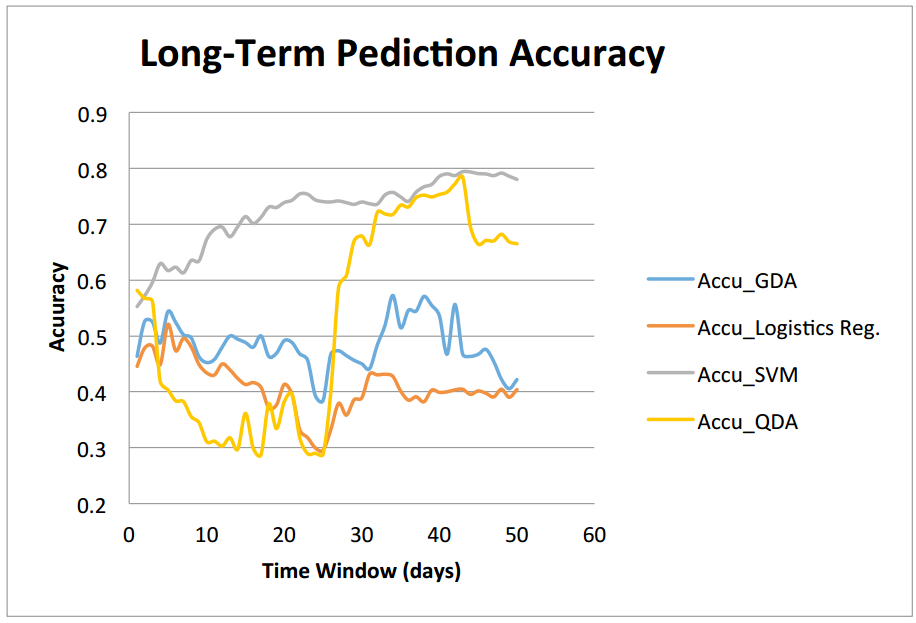
\includegraphics[height=3.5in, keepaspectratio=true]{longtermmodel.png}
\caption{Đồ thị đánh giá mô hình Dài hạn}
\end{figure}\\
Hai mô hình với hai kết quả, ta thấy ở mô hình Dài hạn hai giải thuật SVM và 
QDA cho kết quả Accuracy gần bằng 80\% với $n=44$ ngày, so sánh với mô hình 
Ngày tiếp theo Accuracy gần bằng 60\% ta có thể thấy mô hình dài hạn cho kết 
quả có ý nghĩa hơn. Nhưng một hạn chế rất lớn của công trình này, nhóm tác giả 
chỉ sử dụng một tham số đánh giá duy nhất là Accuracy mà bỏ qua Precision và 
Recall. Việc đánh giá chỉ dựa trên duy nhất một tham số sẽ không thể tổng quát 
được kết quả đầu ra, vì vậy mà dẫn đến nguy cơ không phát hiện các vấn đề về 
lệch dữ liệu hoặc overfitting.\\\\ 
Tổng quan qua hai công trình và tham khảo một số công trình khác, nhận thấy 
đa số các hướng tiếp cận đều đi theo một phương pháp tổng quát chung, nó bao gồm các bước 
cơ bản như:
\begin{enumerate}
\item Xây dựng không gian vector thuộc tính phù hợp với tính chất bài toán
\item Sử dụng các giải thuật phân lớp điển hình trong Máy học như là 
SVM, LR ...
\item Đánh giá giải thuật bằng các tham số Accuracy, Recall, Precision.
\end{enumerate}
Từ những đục kết trên, bản thân nhận thấy các bước trên cũng chính là phương pháp 
nên dùng để tiếp cận đề tài. Ngoài ra, nhận thấy ở hai công trình trên chưa 
hề sử dụng một giải thuật rất được phổ biến hiện nay, nó nổi lên như một đại 
diện của Học sâu - Deep Learning đó là MNN. Do đó mà luận văn này sẽ sử dụng 
MNN như là một giải thuật bổ sung trong quá trình so sánh và đánh giá so với 
các giải thuật phân lớp khác. 
% %====================== Ly thuyet ==================
\chapter{Nền tảng lý thuyết}
\section{Bitcoin}
Các hình thức thương mại trên Internet ngày này hầu như đều dựa vào một tổ chức 
bên thứ ba đáng tin cậy để xử lý các hoạt động thanh toán điện tử. Tuy rằng sau 
nhiều năm phát triển, các tổ chức bên thứ ba này đều đã nâng cao mức độ tin cậy, 
an toàn nhưng đa số vẫn còn tồn tại những điểm yếu: không thể tránh khỏi những 
tranh chấp, phí trung gian, đòi hòi phải cung cấp các thông tin cá nhân... Và 
Bitcoin - hệ thống tiền điện tử ngang hàng (A Peer-to-Peer Electronic Cash System) 
được sinh ra để giải quyết các vấn đề trên \cite{BitcoinPaper}.
\subsection{Máy chủ nhãn thời gian - Timestamp Server}
Máy chủ nhãn thời gian hoạt động bằng cách lấy giá trị băm của block liền trước 
và thông tin của block hiện tại, cho qua hàm băm để được một giá trị băm mới. 
Giá trị băm sau khi được tính toán sẽ được công bố rộng rãi và giá trị băm này 
chứng minh rằng block tồn tại, các block được nối với nhau thành một chuỗi xác 
định.\\
\begin{figure}[h!]
\centering
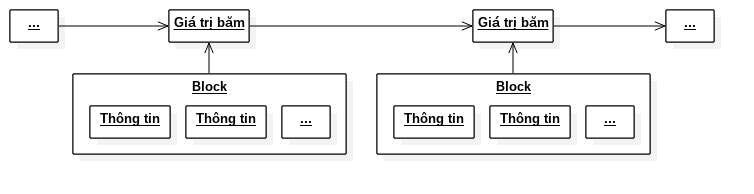
\includegraphics[height=1.45in, keepaspectratio=true]{timestampserver.png}
\caption{Máy chủ nhãn thời gian}
\end{figure}\\
\subsection{Giao dịch - Transaction (trên Blockchain)}
Bitcoin tổ chức các giao dịch bằng cách xây dựng một chuỗi các chữ ký số. Một 
địa chỉ có chứa một lượng BTC được gọi là một chủ sở hữu, một chủ sở hữu 
chuyển một lượng BTC cho một chủ sở hữu khác - người thụ hưởng - bằng cách ký 
lên giá trị băm (hash), trong đó giá trị băm là kết quả sau khi đi qua hàm băm
của tổ hợp giá trị băm giao dịch trước với địa chỉ người thụ hưởng.\\
\begin{figure}[h!]
\centering
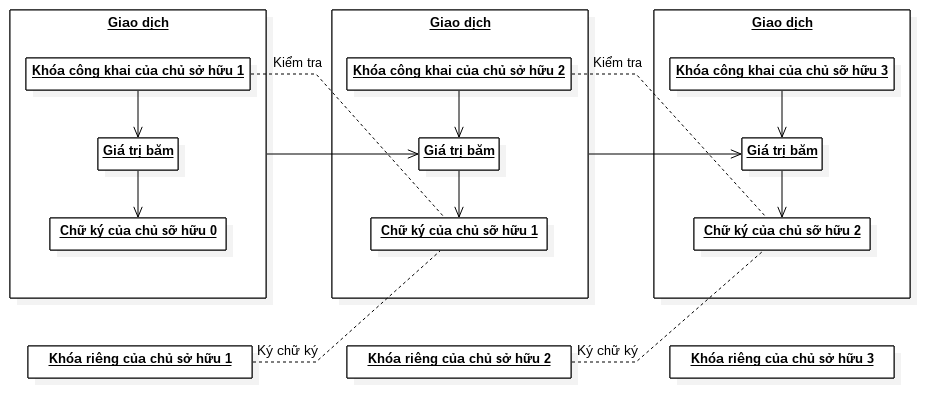
\includegraphics[height=2.45in, keepaspectratio=true]{transaction.png}
\caption{Giao dịch}
\end{figure}\\
\subsection{Proof-of-Work}
Proof-of-Work được hiểu là bằng chứng để chứng minh quá trình lao động, nó dùng 
để kiểm tra quá trình tạo ra kết quả hợp lệ là một quá trình ``lao động'' có 
sử dụng và tiêu tốn tài nguyên.\\\\
Proof-of-Work được sử dụng trong Bitcoin có cơ chế dựa trên hàm băm, ví dụ như 
SHA-256. Quá trình proof-of-work là quá trình đi tăng một con số - gọi là số 
$nonce$ - sao cho giá trị băm của số $nonce$ này cho kết quả đầu ra phải thỏa 
mãn tồn tại $n$ bit 0 ở vị trí đầu, với $n$ xác định và được gọi là số bit 0 
yêu cầu.
\subsection{Blockchain}
Blockchain được hình thành dựa trên sự kết hợp giữa máy chủ nhãn thời gian và 
proof-of-work. Blockchain là một chuỗi các block được kết nối một cách luận lý 
với nhau thông qua các mỗi quan hệ toán học và mật mã, các quan hệ này đảm bảo 
cho hệ thống luôn đúng đắn, không thể sửa và dễ dàng để kiểm tra. Block mới được 
sinh ra phải dựa trên quá trình proof-of-work.\\\\
Quá trình hình thành blockchain được bắt đầu bằng proof-of-work, các peer sẽ đi
tìm số $nonce$ sao cho sau khi cho qua hàm băm kết quả đạt được là một giá trị 
băm thỏa mãn số bit 0 yêu cầu. Số $nonce$ vừa được tìm ra sẽ được đưa và block
mới cùng với các thông tin khác như: thông tin các giao dịch, giá trị băm của 
block kề trước... Tiếp tục như vậy, các block mới được sinh ra và được kết nối 
với block cuối cùng của chuỗi.\\
\begin{figure}[h!]
\centering
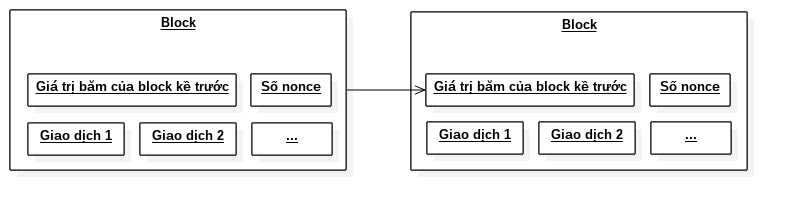
\includegraphics[height=1.5in, keepaspectratio=true]{blockchain.png}
\caption{Blockchain}
\end{figure}\\
Vì hệ thống có tính phân tán nên trên toàn mạng sẽ có nhiều phiên bản của blockchain,
cũng chính vì thế để giải quyết tính đồng nhất, chỉ blockchain có độ dài lớn 
nhất mới được xem là blockchain hợp lệ. Đồng thời để kiểm soát được tốc độ sinh
block mới, hệ thống sẽ quy định một độ khó, nếu toàn mạng có tốc độ sinh block 
(số block được sinh ra trong một giờ đồng hồ) cao hơn mức quy định, độ khó sẽ tăng lên 
để điều chỉnh lại tốc độ của toàn mạng.
\subsection{Mạng - Network}
Mỗi thành viên (máy tính, phần cứng ASIC, thiết bị di dộng... ) khi tham gia vào quá 
trình tính toán của toàn mạng thì sẽ được xem như một node. Toàn mạng sẽ hiện thực hệ 
thống bằng cách thực hiện các bước như sau:
\begin{enumerate}
\item Một gia dịch mới được truyền đi cho tất cả các node (broadcast).
\item Mỗi node sẽ lựa chọn và thu thập các giao dịch để đưa vào block.
\item Mỗi node sẽ thực hiện proof-of-work, tìm ra số $nonce$.
\item Khi một node hoàn thành proof-of-work, node này sẽ đóng block và truyền 
đi toàn tất cả các node khác.
\item Các node khác sẽ kiểm tra thông tin của block nhận được (thông tin các 
transaction, thông tin proof-of-work...) và chấp nhận block này nếu tất cả 
các thông tin đều được kiểm tra chính xác.
\item Các node sẽ thể hiện sự chấp nhận của mình bằng cách thực hiện proof-of-work 
để sinh ra block mới block này sẽ được gắn vào liền sau block mà node đã chấp nhận 
(thêm giá trị băm của block trước mà node chấp nhận vào trong block mới sinh ra).
\end{enumerate}
Lưu ý, một giao dịch mới không nhất thiết phải được truyền đến tất cả các node. 
Chỉ cần việc truyền đến số node đủ nhiều để đảm bảo việc sẽ được đưa vào một block 
và được đóng trong blockchain với độ dài lớn nhất. Cũng như vậy đối với block, 
block không nhất thiết phải được truyền đến tất cả các node, khi một node nhận 
được một block kế block bị thiếu, bằng quá trình kiểm tra node có thể biết được 
và yêu cầu các node khác trong mạng gửi cho node này block bị thiếu sót.
\subsection{Phần thưởng khích lệ}
Trong tập các giao dịch được đóng trong một block sẽ luôn tồn tại một giao dịch 
đặc biệt, giao dịch khác với các giao dịch bình thường, nó không có người chủ 
sở hữu mà chỉ có người thụ hưởng. Điều này giải thích cách mà BTC mới được sinh 
ra, cứ mỗi block được tìm ra nhờ quá trình proof-of-work sẽ có một lượng BTC 
được sinh ra và chính là phần thưởng cho người tạo ra block, điều này đồng nghĩa 
địa chỉ người thụ hưởng chính là địa chỉ của người tạo ra block.\\\\
Ngoài ra, phần thưởng khích lệ khi tạo ra được một block còn bao gồm cả phí giao 
dịch từ các giao dịch đã được đóng trong block. Phí giao dịch thường rất nhỏ và
không đáng kể ở thời điểm hiện tại.
\subsection{Tổ chức lưu trữ thông tin giao dịch}
Đối với các node là các hệ thống máy tính lớn, khả năng lưu trữ và xử lý mạnh thì 
việc lưu một block với đầy đủ các thông tin không gặp nhiều vấn đề. Nhưng đối 
với các thiết bị di động hoặc các thiết bị khác với tài nguyên lưu trữ và xử lý 
tương đối hạn hẹp thì việc lưu một blockchain đầy đủ là khá khó khăn.\\\\
Cây Merkle là một cấu trúc tổ chức dữ liệu, trong đó giá trị của node cha sẽ 
là kết quả hàm băm tất cả các giá trị (nhãn hoặc dữ liệu) của nốt con. Các nốt 
không phải lá thì giá trị sẽ là nhãn - kết quả hàm băm, các nốt lá sẽ có giá trị 
là dữ liệu cần được tổ chức.\\\\
Bitcoin sử dụng cây Merkle để tổ chức các giao dịch, nốt cao nhất của cây được 
gọi là giá trị băm gốc (Root hash) và giá trị này sẽ được lưu vào block. Ở đây,
ta thấy việc thay đổi bất kỳ một giá trị nào trong cây cũng sẽ dẫn đến việc thay 
đổi giá trị băm gốc, vì thế giá trị băm gốc khi được lưu vào block nó có chức 
năng dùng để kiểm tra lại các giao dịch trong block đó là toàn vẹn hay không.\\
\begin{figure}[h!]
\centering
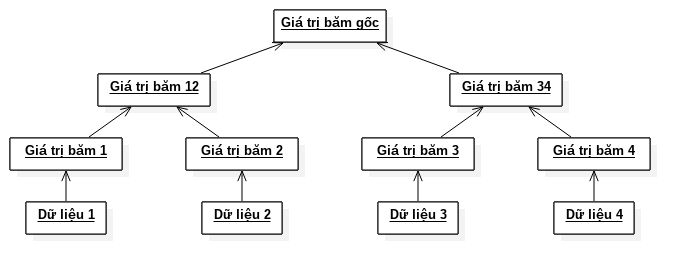
\includegraphics[height=2.25in, keepaspectratio=true]{merkletree.png}
\caption{Cây Merkle}
\end{figure}
\begin{figure}[h!]
\centering
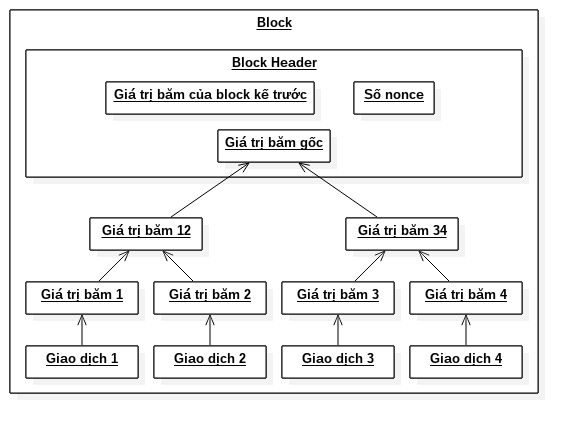
\includegraphics[height=3.75in, keepaspectratio=true]{block.png}
\caption{Cấu trúc tổ chức giao dịch trong một block}
\end{figure}\\
Một node với tài nguyên hạn chế khi muốn lưu blockchain không nhất thiết phải 
lưu đầy đủ thông tin của từng block trong blockchain, thay vào đó node có thể 
lược bỏ các thông tin về giao dịch được đóng trong block và chỉ lưu giá trị băm 
gốc của các giao dịch này. Điều này làm giảm chi phí về lưu trữ nhưng vẫn đảm 
bảo được tính toàn vẹn, khi muốn xác minh bất kỳ giao dịch nào, node chỉ cần 
yêu cầu các giao dịch trong block và tính toán lại giá trị băm gốc, nếu giá trị 
băm nào giống với giá trị băm gốc được lưu nghĩa là các giao dịch hoàn toàn hợp 
lệ.
\section{Một số khái niệm về tài chính}
Vì luận văn này đang giải quyết một bài toán về kinh tế nên để hiểu được công 
việc, ta cần nắm được các ý niệm cơ bản về kinh tế.
\subsection{Phiên giao dịch và các giá trị cơ bản}
Gọi T là một mốc thời gian bất kỳ, P là khoảng thời gian được chọn là một phiên 
giao dịch. Ta có thể nói một cách đơn giản là phiên giao dịch được mở tại thời 
điểm T và được kết thúc tại thời điểm T + P.\\\\
Cụ thể, giả sử chọn mốc mở phiên là 9:00 am và phiên giao dịch có thời hạn là 
30 phút, điều đó có nghĩa là kết thúc phiên giao dịch sẽ là 9:30 am.\\\\
Ngoài ra:
\begin{itemize}
\item Giá mở phiên: là giá bán của một giao dịch gần nhất sau thời điểm T. Ví dụ tại thời 
điểm 9:01 am có một giao dịch bán 1 BTC là \$779 và trong khoảng thời gian 9:00 am 
đến 9:01 am không hề có bất kỳ giao dịch nào khác ngoại trừ giao dịch này, thì ta có thể 
nói giá mở phiên sẽ là \$779.
\item Giá đóng phiên: là giá bán của một giao dịch gần nhất trước thời điểm T + P.
\item Giá phiên cao nhất: là giá bán cao nhất của một giao dịch trong khoảng thời gian diễn ra phiên 
giao dịch, cụ thể là từ thời điểm T đến thời điểm T + P. Ví dụ, trong khoảng thời gian 9:00 am (thời điểm 
mở phiên) đến thời gian 9:30 am (thời điểm đóng phiên) có một giao dịch BTC với giá là 
\$801 và là giao dịch có giá trị cao nhất. Vậy ta có thể nó giá phiên cao nhất là 
\$801.
\item Giá phiên thấp nhất: là giá bán thấp nhất của một giao dịch trong khoảng thời gian diễn ra phiên 
giao dịch, cụ thể là từ thời điểm T đến thời điểm T + P.
\item Lượng giao dịch: tổng giá trị USD được dùng để  mua/bán BTC trong một phiên giao dịch.
\item Trung bình giao dịch: giá trị USD trung bình của tất cả các giao dịch diễn 
ra trong khoảng thời gian một phiên giao dịch.
\end{itemize}
\subsection{Rate of Change}
Đại lượng đo sự khác nhau của giá tại phiên thứ x so với n phiên trước đó. 
Giá sử $P(x)$ là giá của phiên thứ $x$ thì:
\[ ROC_{n}(x)=\frac{P(x)-P(x-n)}{P(x-n)}\]
Nếu $ROC > 0$ thì giá thị trường đang có xu hướng đi lên (tăng giá).
Ngược lại, với $ROC < 0$ thì giá thị trường đang có xu hướng giảm xuống.
\subsection{Stochastic Oscillator}
Đại lượng dùng để đo xu hướng mua/bán của thị trường tại thời điểm phiên x thông 
qua n phiên trước đó. Giả sử:\\\\
\tab $L_{n} = $ giá phiên thấp nhất trong n phiên\\
\tab $H_{n} = $ giá phiên cao nhất trong n phiên\\
\tab $P(x) = $ giá của ngày x\\
\[\%K=\frac{P(x)-L_{n}}{H_{n}-L_{n}}\]
Nếu $ \%K $ nhỏ hơn 20 thì thị trường đang có xu hướng mua vào và nếu lớn hơn 
80 thì thị trường đang có xu hướng bán ra.


\section{Máy học}

\subsection{Khái niệm cơ bản}
\subsubsection{Máy học}
Máy học có hai cách định nghĩa chính và đang được chấp nhận phổ biến:
\begin{itemize}
  \item Theo Arthur Samuel: \textit{``Là một lĩnh vực nghiên cứu mà nó cung cấp cho
  máy tính khả năng học hỏi mà không cần lập trình một cách tường minh.''}
  \item Theo Tom Mitchell: \textit{``Một chương trình máy tính được chấp nhận
  là học hỏi được kinh nghiệm E bằng cách thực hiện một vài tác vụ T theo phép đo hiệu
  năng P, nếu và chỉ nếu việc thực thi các tác vụ trong T được đo bởi phép đo P
  đem lại kết quả là kinh nghiệm E được cải thiện.''}
\end{itemize}
\subsubsection{Supervised Learning - Học có giám sát}
Chúng ta được cho một tập dữ liệu đã biết với các input và output tương ứng
nhau. Ý tưởng là chúng ta sẽ đi tìm mối quan hệ giữa input và output đó chính là
Supervised Learning.\\\\
Vấn đề của Supervised Learning được phân loại thành hai
vấn đề chính là “Regression” và “Classification”. Trong vấn đề “Regression”,
chúng ta sẽ cố gắng dự đoán kết quả output tiếp theo một cách liên tục, nghĩa là
chúng ta đi tìm ra một hàm đầu ra liên tục tổng quát với biến là các thuộc tính
đầu vào. Còn với vấn đề “Classification”, chúng ta thay vì cố gắng dự đoán kết
quả liên tục thì ta sẽ đi dự đoán chúng theo hướng rời rạc, hiểu theo một cách
khác là chúng ta đi tìm một phép phân loại rời rạc cho output với các biến
input.
\subsubsection{Unsupervised Learning - Học không giám sát}
Học không giám sát cho phép chúng ta tiếp cận các vấn đề mà ta chưa hề hoặc biết
rất ít kết quả của chúng ta sẽ trông như thế nào. Chúng ta có thể xây dựng cấu
trúc của dữ liệu mà không cần thiết phải biết ảnh hưởng của các biến đó.\\\\
Chúng ta thực hiện việc này dựa trên ý tưởng gom cụm dữ liệu bằng cách xem xét
mối quan hệ giữa các thuộc tính của dữ liệu. Các hướng tiếp cận dựa trên nhưng 
phương pháp như vậy thường được gọi là “Clustering”.

\subsection{Thông số đánh giá}
Có ba tham số cơ bản dùng để xem xét và đánh giá giải thuật trong Máy học.
Gọi:
\begin{itemize}
\item True positive là TP
\item False positive là FP
\item True negative là TN
\item False negative là FN
\end{itemize}
Thì:\\
\[
  Accuracy = \frac{TP+TN}{TP+FP+TN+FN}
\]
\[
  Precision = \frac{TP}{TP+FP}
\]
\[
  Recall = \frac{TP}{TP+FN}
\]\\
\begin{figure}[h!]
\centering
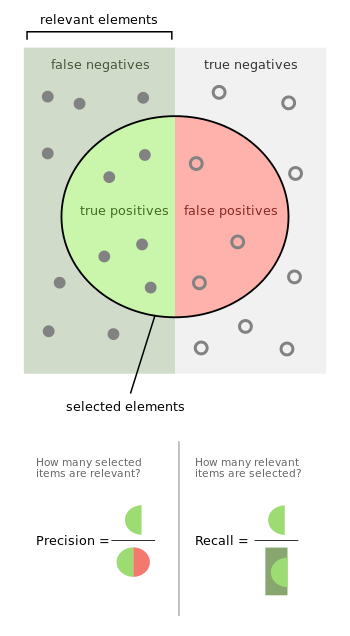
\includegraphics[height=7in, keepaspectratio=true]{precision_recall.png}
\caption{Validation Parameters}
\end{figure}\\
\subsection{Neural Network - Deep Learning}
Deep Learning nói chung và Neural Network nói riêng là hai phạm trù xuất hiện 
không lâu đối với Máy học, đại diện cho hướng tiếp cận gần với 
cái nhìn thực tế, học nhiều cấp và học từ bản chất dữ liệu. Deep Learning 
thường giải quyết rất tốt với các loại dữ liệu mang tính ``con người'' như 
hình ảnh, âm thanh ... \cite{NeuralNetworksandDeepLearning} 
\subsubsection{Ý tưởng giải thuật}
Bộ não con người là một trong những phát minh vĩ đại nhất của tự nhiên, nó 
có thể giải quyết các bài toán mà đối với máy tính là cực kỳ phức tạp chỉ trong 
vài giây hoặc kể cả là vài phần giây, các khả năng phán đoán, học hỏi, tích lũy 
kinh nghiệm đó chính là điều tuyệt diệu của bộ não con người. Và các nhà khoa học 
khao khát một thứ gì đó trong giới máy tính có khả năng như vậy.\\\\
Dựa trên ý tưởng kết cấu của bộ não gồm hàng tỷ neural liên kết lại với nhau, 
mỗi neural chỉ đưa ra một tín hiệu hết sức đơn giản, nhưng khi hàng tỷ neural liên kết 
hình thành nên một hệ thống phức tạp thì từ đó có khả năng giải quyết các vấn đề 
phức tạp. Các nhà khoa học máy tính, đã cố gắng định nghĩa một neural đơn lẻ 
trong phạm trù máy tính và được gọi là perceptron, từ đó kết nối lại với nhau 
để tạo nên một hệ thống hữu hạn các perceptron có khả năng giả lập một bộ não 
người - mạng neural nhân tạo.

\subsubsection{Cấu trúc một Perceptron}
Một perceptron sẽ có các input $x_1, x_2, ...$ và output sẽ là một giá trị 
nhị phân.\\
\begin{figure}[h!]
\centering
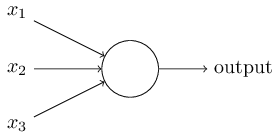
\includegraphics[height=1.5in, keepaspectratio=true]{perceptron.png}
\caption{Perceptron}
\end{figure}\\
Một ví dụ đơn giản dựa vào hình trên, ta thấy perceptron này có 3 input là 
$x_1, x_2, x_3$ , giả sử đi kèm với mỗi input sẽ có một giá trị trọng 
số $w_1, w_2, w_3$. Output được định nghĩa là 0 và 1, nhận giá trị 0 
khi $\sum_j w_j x_j$ nhỏ hơn giá trị ngưỡng và 1 khi lớn gơn giá trị ngưỡng.\\\\
Biểu diễn đại số:\\
\[
  output = 
  \bigg\{
    _{0 \quad if \, \sum_j w_j x_j \, \leq \, threshold}
    ^{1 \quad if \, \sum_j w_j x_j \, > \, threshold}
\]
Các hàm số như trên được gọi là activation function, có nhiều loại activation
 function khác nhau như: $sigmoid , tang ...$ 

\subsubsection{Multilayer Neural Network}
Hiển nhiên, một perceptron không thể mô phỏng nên được một bộ não người, để 
có thể đưa ra một quyết định tương tự như bộ não người các perceptron này cần 
được kết nối với nhau thành một mạng lưới - Multilayer Neural Network.\\
\begin{figure}[h!]
\centering
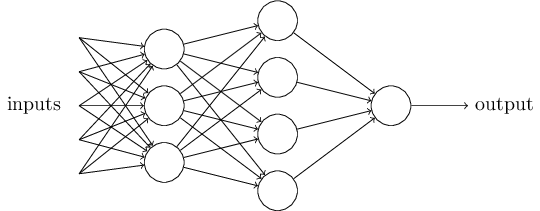
\includegraphics[height=2in, keepaspectratio=true]{multilayerneuralnetwork.png}
\caption{Multilayer Neural Network}
\end{figure}\\
Multilayer Neural Network được cấu thành bằng cách sắp xếp các perceptron thành 
từng lớp. Các perceptron ở mỗi lớp sẽ kết nối với tất cả các perceptron ở các 
lớp liền kề, cột những perceptron đầu tiên được gọi là input layer, chúng có 
chức năng tiếp nhận các input để cho ra các output. Các output ở lớp trước sẽ chính là 
input cho các perceptron ở lớp tiếp theo. Các perceptron ở lớp cuối cùng được gọi là 
output layer, trong trường hợp này đặc biệt chỉ có duy nhất một perceptron. Còn 
lại các lớp perceptron khác được gọi là hidden layer.\\\\
Giả sử input của perceptron là $x_1, x_2, ...$ tương ứng là đó là các trọng 
số $w_1, w_2, ...$. Thêm vào đó định nghĩa về bias, ở đây bias là một giá trị 
đại diện độ lệch của từng perceptron và được ký hiệu $b_1, b_2, ...$. Ta có biểu diễn của activation 
function:\\
\[
  output = 
  \bigg\{
    _{0 \quad if \, \sum_j w_j x_j + b_i\, \leq \, 0}
    ^{1 \quad if \, \sum_j w_j x_j + b_i\, > \, 1}
\]
Ví dụ:\\
\begin{figure}[h!]
\centering
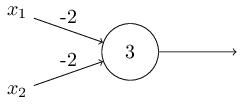
\includegraphics[height=1in, keepaspectratio=true]{exmln.png}
\caption{Perceptron with Bias example}
\end{figure}\\
Ta có $w_1=w_2=-2$ và $b=3$, khi đó nếu input $x_1=1,\, x_2=0$ suy ra $ 
w_1*x_1+w_2*x_2+b=(-2)*1+(-2)*0+3=1$, ta có thể chọn $threshold=0$ vì $1>0$
nên $output=1$.

\subsubsection{Sigmoid Function - Hàm Sigmoid}
Với dạng activation function được định nghĩa ở trên, giá trị của activation 
function gần như không có giới hạn. Vậy tại sao việc không có giới hạn lại 
cần được quan tâm. Trong một trường hợp cụ thể, với việc sử dụng activation 
function như trên có thể dẫn đến trường hợp đầu ra của một perceptron sẽ nhận 
giá trị rất lớn - giả sử là 1000, những một perceptron khác sẽ nhận giá trị rất 
bé - giả sử 0.001. Vì thế khi đến lớp tiếp theo thì gần như perceptron cho kết 
quả đầu ra là giá trị bé sẽ mất đi độ ảnh hưởng và làm mất cân đối cho toàn mạng.\\\\
Do đó để giới hạn giá trị của activation function chúng ta sẽ sử dụng hàm sigmoid. 
Sigmoid function được định nghĩa như sau:\\
\[
  \sigma(z)=\frac{1}{1+e^{-z}}
\]
Áp dụng Sigmoid function vào activation function ta có activation function dạng
sigmoid và khi đó activation function của chúng ta sẽ có dạng:\\
\[
  \frac{1}{1+exp(-\sum_j w_j x_j -b)}
\]
Lúc này ta có một activation function có giá trị được giới hạn trong khoảng 
từ 0 đến 1. Nhưng chú ý, giá trị của activation function là liên tục, để rời 
rạc hóa giá trị của activation function ta có thể sử dụng một phương pháp 
quen thuộc - sử dụng threshold. Điển hình ta chọn threshold = 0.5, nếu lớn hơn 
thì activation function sẽ nhận 1 và ngược lại sẽ nhận 0.\\\\
Để hiểu rõ hơn tại sao chúng ta quan sát hai đồ thị của sigmoid function và 
activation function có dạng sigmoid và đã được rời rạc hóa giá trị:\\
\begin{figure}[h!]
\centering
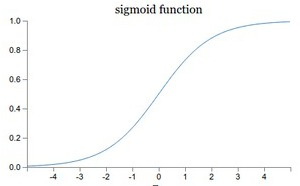
\includegraphics[height=2.5in, keepaspectratio=true]{sigmoid.jpg}
\caption{Sigmoid Function}
\end{figure}\\
\begin{figure}[h!]
\centering
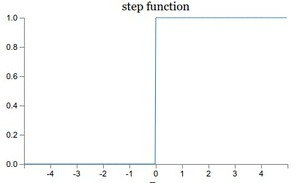
\includegraphics[height=2.5in, keepaspectratio=true]{step.jpg}
\caption{Step Function}
\end{figure}\\

\subsubsection{Giải thuật Backpropagation}
Sau khi đã có xây dựng thành công một mô hình Multilayer Neural Network, công 
việc cuối cùng là cung cấp khả năng tự học hỏi từ đó để bản thân mạng có thể 
tự xây dựng mô hình và đưa ra các quyết định cụ thể.\\\\
Cụ thể, khi nhìn lại một Multilayer Neural Network với activation function là 
sigmoid function thì các tham sô $w, b$ là chưa biết và việc cung cấp khả năng 
tự học hỏi chính là cung cấp một giải thuật giúp mạng tìm được các tham số 
$w, b$ với một tập kinh nghiệm - hay tập huấn luyện - ${x, y}$ cụ thể, trong 
đó $x$ là input và $y$ là output tương ứng với từng bộ $x$. Giải thuật backpropagation 
là một trong nhưng giải thuật chúng ta cần tìm.\\\\
Trước tiên chúng ta cần đi qua một số ký hiệu:\\\\
\begin{itemize}
\item $w$ là vector của các giá trị trọng số\\ 
\[ w =
\begin{bmatrix}
w_1\\
\vdots\\
w_n
\end{bmatrix}
\]
\item $b$ là vector của các giá trị bias\\ 
\[ b =
\begin{bmatrix}
b_1\\
\vdots\\
b_m
\end{bmatrix}
\]
\item $\sigma$ là sigmoid function
\item $a(\sigma)$ là activation function có dạng sigmoid
\end{itemize}
Biểu diễn activation function:\\
\begin{figure}[h!]
\centering
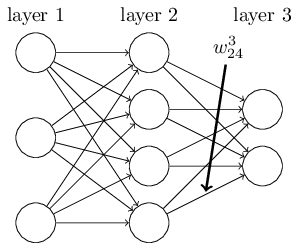
\includegraphics[height=2in, keepaspectratio=true]{exw.png}
\caption{Weight Notation example}
\end{figure}\\
Ví dụ như hình trên, trọng số xuất phát từ perceptron thứ 4 thuộc layer thứ 
2 và kết thúc tại perceptron thứ 2 thuộc layer thứ 3 được ký hiệu là 
$w_{24}^3$.\\\\
Tương tự như vậy với bias và activation function của perceptron thứ j thuộc layer 
thứ l của mạng sẽ được kí hiệu thứ tự là $b_j^l,\,a_j^l$. Ví dụ, bias của perceptron 
thứ 3 thuộc layer thứ 2 sẽ là $b_3^2$ và activation function của perceptron thứ 
1 thuộc layer thứ 3 sẽ là $a_1^3$.\\
\begin{figure}[h!]
\centering
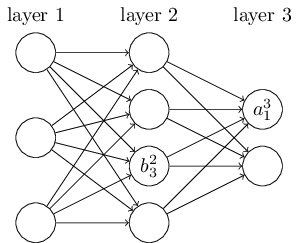
\includegraphics[height=2in, keepaspectratio=true]{exb.png}
\caption{Bias Notation example}
\end{figure}\\
Lúc này ta có biểu diễn toán học đầy đủ của activation function:\\
\[
  a_j^l=\sigma(\sum_k w_{jk}^l a_k^l-1 + b_j^l)
\]
Với ký hiệu vector ta có thể tổng quát phát biểu với dạng:\\
\[
  a^l=\sigma(w^l a^{l-1} + b^l)
\]
\textbf{Cost function:} Trước khi đi vào hiểu được backpropagation có thể làm gì, 
chúng ta cần phải biết một định nghĩa cost function. Vậy cost function là gì? 
Đúng theo tên của hàm, nó dùng để đo lường chi phí của thuật toán. Chi tiết:\\
\[
  C=\frac{1}{2n}\sum_x\|y(x)-a^L(x)\|^2
\]
Ta có thể thấy, dạng hàm số trên hết sức quen thuộc với định nghĩa độ lệch chuẩn 
trong xác suất thống kê nhưng đã được biến đổi một chút. Thay vì giá trị kỳ vọng 
và các điểm xác suất, cost function sử dụng giá trị thực tế $y$ của tập dữ liệu 
và giá trị $y=a$ là giá trị $y$ tính toán được từ $x$ với $w$ và $b$. Vậy ta 
có thể hiểu được, cost function tính toán độ sai lệch của giá trị $a$ so với 
$y$ kỳ vọng thực tế. Do đó, cost function càng nhỏ thì biểu diễn giá trị của 
Multilayer Neural Network sẽ càng gần với thực tế.\\\\
Để tìm được giá trị cực tiểu cho cost function ta sẽ thực hiện vòng lặp:\\
\[
  w_ij^{(l)}:=w_ij^{(l)}-\eta\frac{\sigma}{\sigma w_ij^{(l)}}C(w,b)
\]
\[
  b_i^{(l)}:=b_i^{(l)}-\eta\frac{\sigma}{\sigma b_i^{(l)}}C(w,b)
\]

Trong đó $\eta$ là learning rate - tỉ lệ học, việc hội tụ về giá trị cực tiểu với 
tốc độ và độ chính xác phụ thuộc vào tỉ lệ này.\\\\
Vậy, đi qua một quá trình tìm hiểu về Multilayer Neural Network, ta có thể hiểu 
được việc học hỏi kinh nghiệm của mạng cốt lõi vẫn là việc tìm ra bộ $w$ và $b$ 
tương ứng với ${x, y}$ của bộ dữ liệu luyện tập, và để tìm ra được $w$ và $b$ 
ta có thể sử dụng giải thuật backpropagation.
\chapter{Phân tích và thiết kế hệ thống}
\section{Xây dựng MNN}
\subsection{Xây dựng dữ liệu luyện tập}
Một trong những yếu tố hết sức quan trọng trong Máy học đó chính đặc trưng 
- feature. Đặc trưng chính là các giá trị thuộc tính đại diện cho tập dữ liệu 
luyện tập, ví dụ chúng ta có tập dữ liệu về loài chim thì có thể nói đặc trưng 
chính là các thông số như: độ dài sải cánh, màu lông, vùng sinh sống... Một 
giải thuật có thể học được ``kinh nghiệm'' nhanh hay chậm, chính xác hay sai lệch 
phụ thuộc rất nhiều vào yếu tố đặc trưng. Vì vậy quá trình khai phá dữ liệu 
chính là đi tìm kiếm các đặc trưng có ý nghĩa cho giải thuật máy học và là 
công việc hết sức quan trọng.\\\\
Tập dữ liệu về các phiên giao dịch Bitcoin được thu thập từ ngày 20/2/2015 đến 
ngày 29/10/2016 và có tổng cộng 29634 mẫu (mỗi mẫu là đại diện của một phiên 
giao dịch), nguồn dữ liệu được lấy thông qua API của sàn giao dịch Poloniex.\\\\
Gọi $S$ là đại diện cho một phiên giao dịch, các đặc trưng được xây dựng như 
sau:
\begin{itemize}
    \item 10 feature RDP: $\{ \: loop\{ RDP_1(S_{i+j})\}_i \: \}_j$ Với 
    $i \in [0:9], \: j \in [0:29634]$
    \item 1 feature SO. Với $ j \in [0:29625] $:\\
    \[
        \{ \%K_j = \frac{P(j+9)-L_{10}}{H_{10}-L_{10}} \}_j
    \]
    \item 1 feature ROC. Với $ j \in [0:29625] $:\\ 
    \[
        \{ ROC_{10}(j)= \frac{P(j+9) - P(j)}{P(j)} \}_j
    \]
\end{itemize}
Ở đây, chúng ta chọn mỗi vector đặc trưng được hình thành bởi 10 phiên giao 
dịch. Các giá trị SO và ROC đều được tính trong thời gian là 10 phiên giao dịch.
Sau khi đã có tập luyện tập (tập hợp các vector đặc trưng), ta cần nhãn - label 
để phân lớp tập luyện tập. Nhãn được định nghĩa như sau, nếu giá BTC ở phiên 
thứ 11 lớn hơn phiên thứ 10 thì nhãn sẽ là 1, ngược lại sẽ là 0 (Phiên 11 chính 
là phiên thứ 1 của nhóm 10 phiên liền sau nhóm 10 phiên hiện đang xét).\\
\[
    label_i = \bigg \{ _{0 \quad if \: P_i(10) \: \leq \: P_{i+1}(1)} ^{1 \quad if \: P_i(10) \: > \: P_{i+1}(1)}
\]
\subsection{Học giải thuật}
Bên cạnh chạy giải thuật MNN, chúng ta sẽ chạy các giải thuật khác nhằm so sánh 
và đánh giá giải thuật chính.\\\\
Các giải thuật được chọn để so sánh với giải thuật chính: SVM, KNN, LR. Sau khi 
chạy xong ta ghi nhận kết quả của các giải thuật được đề cập dưới dạng các tham 
số đánh giá sau: Accuracy, Recall, Precision.\\\\
Các giải thuật được chạy bằng thư viện scikit-learn phiên bản 0.18.0 với các 
tham số mặc định.
\subsection{Đánh giá giải thuật}
Để có được kết quả đánh giá trên lý thuyết, chúng ta sẽ chia tập dữ liệu ra hai 
phần:
\begin{itemize}
\item Tập huấn luyện: chiếm 7/10 tổng số dữ liệu, dùng để chạy trong quá trình 
học của giải thuật.
\item Tập đánh giá: chiếm 3/10 tổng số dữ liệu, dùng để chạy trong quá trình 
đánh giá giải thuật.
\end{itemize}
Kết quả chạy giải thuật:
\begin{table}[h]
\centering
\begin{tabular}{ |c|c|c|c|c| }
\hline
 & KNN & LR & SVM & MNN \\
\hline
Accuracy & 62.93\% & 66.24\% & 66.40\% & 69.86\% \\
\hline
Precision & 44.69\% & 18.18\% & 0\% & 60.50\% \\
\hline
Recall & 43.62\% & 0.15\% & 0\% & 29.55\% \\
\hline
\end{tabular}
\caption{Bảng đánh giá}
\end{table}\\
Trước tiên theo bảng đánh giá, ta có các giải thuật LR và SVM cho kết quả Accuracy
là gần khoảng 66\%, nhưng khi nhìn vào chi tiết các giá trị Precision và Recall 
ta nhận thấy các giải thuật này hầu như chỉ dự đoán kết quả là nhãn $Down$ cho \
tất cả trường hợp. Điều này hoàn toàn không có ý nghĩa để dự đoán đầu tư.\\\\
Xét đến KNN và MNN, đối với KNN ta có thể thấy giải thuật có xu hướng cân bằng 
các giá trị Accuracy, Precision và Recall. Nhưng đối với MNN, giải thuật có xu 
hướng tối ưu hóa Accuracy và Precision. Vậy câu hỏi đặt ra ở đây là kết quả nào 
có giá trị đầu tư hơn?\\\\
Chú ý đến Recall, dựa theo định nghĩa thì Recall có thể hiểu nếu trong thực tế 
có 10 phiên là $Up$ thì KNN sẽ dự đoán đúng khoảng 4 lần và MNN sẽ dự đoán đúng 
khoảng 3 lần. Điều này có nghĩa là KNN sẽ chiếm ưu thế so MNN khi sử dụng tiêu 
chuẩn là Recall.\\\\
Xét đến Precision, ta có thể hiểu Precision như sau, với 10 lần dự đoán sẽ có 
phiên $Up$ thì KNN sẽ đúng khoảng 4 lần và MNN sẽ dự đoán đúng 6 lần. Giả sử, 
mức độ tin tưởng của chúng ta vào hệ thống là 100\%, cứ mỗi lần hệ thống dự 
đoán có phiên $Up$ thì ta sẽ quyết định đầu tư. Điều đó đồng nghĩa, nếu theo 
KNN sẽ có 6 lần ta chịu lỗ vì hệ thống dự đoán sai và với MNN thì ta sẽ có 4 
lần ta chịu lỗ.\\\\
Quay lại với Recall, giá trị này không đo đạt được việc chúng ta sẽ lợi nhuận 
hoặc thua lỗ ra sao mà thực ra là giá trị đo đạt khả năng tận dụng cơ hội của 
hệ thống.\\\\
Tới lúc này, ta có thể kết luận, bộ tiêu chuẩn chiếm ưu thế cao hơn sẽ là Accuracy 
và Precision. Điều đó cũng có nghĩa là giải thuật MNN có kết quả ý nghĩa hơn so 
với KNN và sẽ được lựa chọn để giải quyết bài toán dự đoán xu hướng giá trị BTC.
\section{Xây dựng hệ thống}
Hệ thống được xây dựng với mục tiêu là một ứng dụng nền web, cung cấp công cụ hỗ 
trợ cho việc dự đoán xu hướng giá trị BTC.
\subsection{Tổng quan hệ thống}
Hệ thống được xem xét và được thiết kế với 3 khối server chức năng:
\begin{itemize}
\item Hệ thống máy chủ máy học - Machine Learning server
\item Hệ thống máy chủ backend - Backend server
\item Hệ thống máy chủ UI frontend - UI Frontend server
\end{itemize}
Các khối hệ thống giao tiếp với nhau bằng API và Socket - đối với các chức năng
chạy thời gian thực.\\
\begin{figure}[h!]
\centering
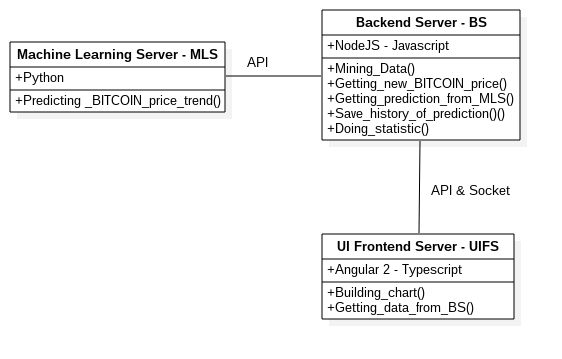
\includegraphics[height=3.5in, keepaspectratio=true]{system.png}
\caption{Cấu trúc quan hệ và chức năng hệ thống}
\end{figure}
\subsection{Hệ thống máy chủ máy học}
Đây là hệ thống cốt lõi của của sản phẩm, nó đảm nhiệm khối chức năng dựa vào 
các tham số được truyền vào để đưa ra giá trị nhãn tương ứng cho bộ tham số 
đó.\\\\
Cụ thể, để đưa ra một dự đoán, hệ thống yêu cầu các tham số đầu vào phải được 
xây dựng theo mô tả tại phần 4.1.1, tổng số đặc trưng là 12.\\\\
Hệ thống máy chủ máy học được chia thành hai phần:
\begin{enumerate}
\item Prediction: bao gồm các chức năng đọc mô hình MNN đã xây dựng, chạy mô 
hình với tham số truyền vào và lấy các kết quả đầu ra.Kết quả đầu ra có giá 
trị nhãn $Up-Down$ và xác suất dự đoán.
\item Django: bao gồm các chức năng để hình thành một API server ví dụ như 
tiếp nhận các yêu cầu thông qua API, phản hồi các yêu cầu...
\end{enumerate}
Vì tính chất hỗ trợ tốt cho Máy học nên Python được lựa chọn là ngôn 
ngữ để phát triển hệ thống này.
\subsection{ Hệ thống máy chủ backend}
Vì bản thân hệ thống máy chủ máy học không có các khối chức năng liên quan đến 
việc lấy dữ liệu giá BTC cũng như khai phá dữ liệu nên hệ thống máy chủ backend 
được xây dựng để thực hiện các chức năng này. Đồng thời, máy chủ backend còn là 
cầu nối giữa trải nghiệm người dùng (hệ thống máy chủ UI frontend) và hệ thống 
máy chủ máy học.\\\\
Để thực hiện được công việc trên, hệ thống bao gồm được xây dựng các chức năng:
\begin{enumerate}
\item Cập nhật giá BTC: thông qua các public API được sàn giao dịch Poloniex 
cung cấp, các hàm lấy giá được chạy liên tục để cập nhật giá BTC mới nhất nhằm 
phục vụ cho quá trình dự đoán (trung bình 20 giây).
\item Khai phá dữ liệu: dữ liệu được các hàm cập nhật giá BTC lấy được vẫn 
còn ở dạng thô, chưa qua xử lý. Khai phá dữ liệu là biến đổi các dữ liệu này 
về các bộ tham số có ý nghĩa với Máy học, các giá trị này mới đích thực 
dùng để làm đầu vào dự đoán xu hướng giá trị BTC.
\item Giao tiếp với hệ thống máy chủ máy học: truyền tham số đi và nhận 
kết quả trả về từ hệ thống máy chủ máy học thông qua API.
\item Lưu trữ và thống kê dữ liệu: thực hiện việc lưu trữ dữ liệu, từ đó tạo 
nên một hệ thống các dữ liệu phục vụ cho việc phân tích, thống kê để cung cấp 
cho người dùng đầu cuối. Đó là các thông tin hết sức quý giá phục vụ cho các 
nhà đầu tư.
\item Giao tiếp với hệ thống máy chủ UI frontend: đưa ra những API chức năng 
nhằm phục vụ cho máy củ UI frontend. Ví dụ như: yêu cầu dữ liệu dự đoán, yêu 
cầu thống kê đúng/sai, yêu cầu dữ liệu giá cho biểu đồ...
\end{enumerate}
Với khả năng xử lý nhanh, được hỗ trợ tốt nên NodeJS được dùng để phát triển 
hệ thống. Đồng thời, cơ sở dữ liệu của hệ thống là MongoDB vì tính linh hoạt 
trong cấu trúc dữ liệu và khả năng mở rộng cao.
\subsection{Hệ thống máy chủ UI frontend}
Hệ thồng UI Frontend Server là một giao diện người dùng, nó cho phép người 
dùng có thể tiếp cận với các chức năng của toàn bộ hệ thống một cách dễ dàng. 
Hệ thống bao gồm nhiều biểu đồ, cũng như tham số cung cấp các thông tin có ý 
nghĩa đầu tư - dự đoán xu hướng giá trị Bitcoin - đồng thời với đó, là các 
thông tin về độ tin cậy của hệ thống, các thống kê về lịch sử dự đoán...\\\\
Một số hình ảnh về hệ thống thực tế.\\
\begin{figure}[h!]
\centering
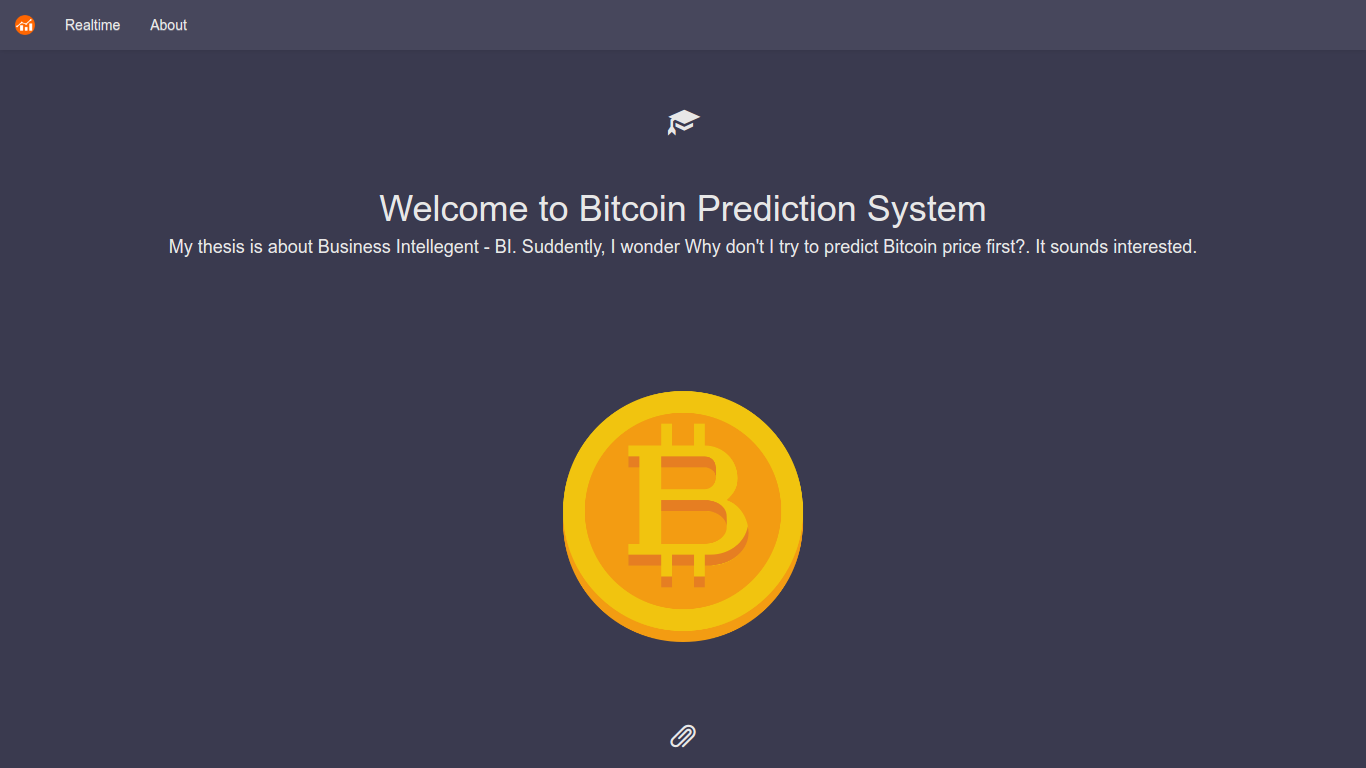
\includegraphics[height=3in, keepaspectratio=true]{1.png}
\caption{Giao diện 1 máy chủ UI frontend}
\end{figure}\\
\begin{figure}[h!]
\centering
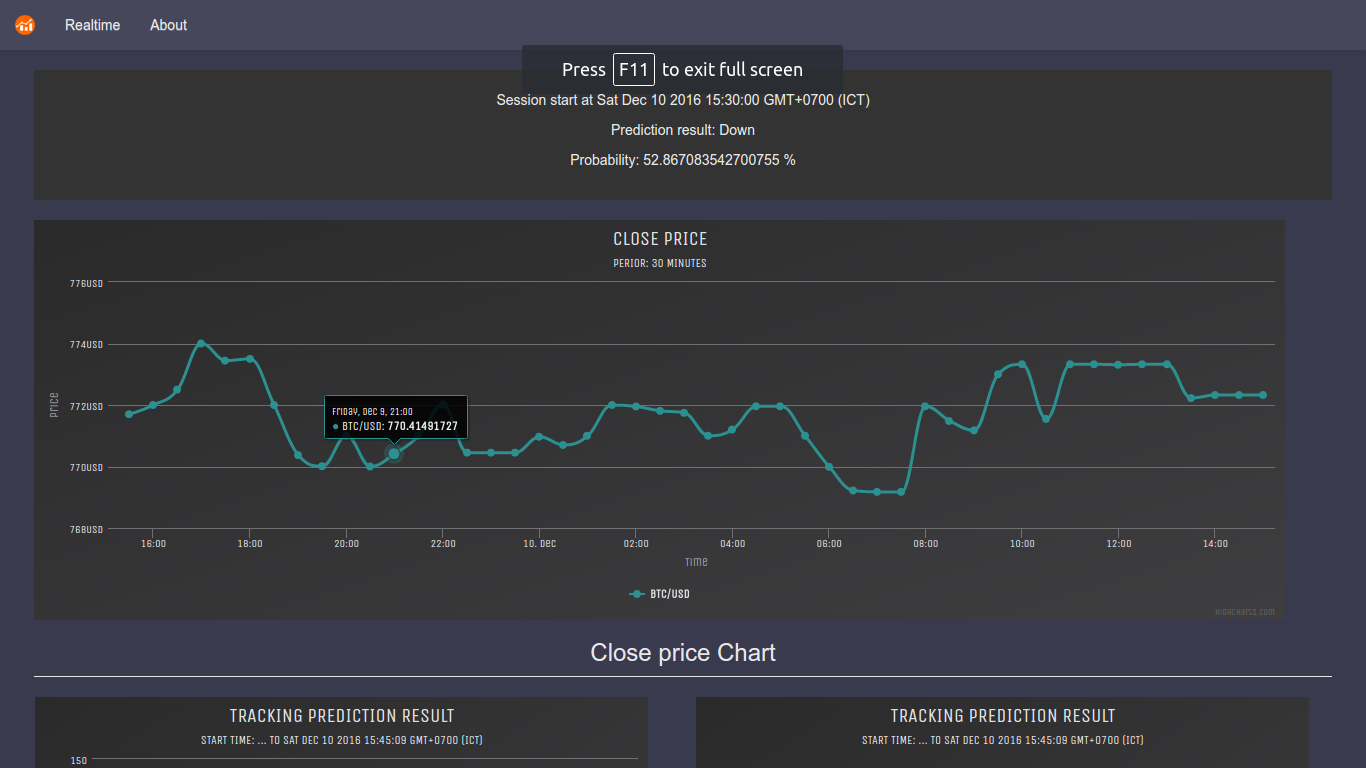
\includegraphics[height=3in, keepaspectratio=true]{2.png}
\caption{Giao diện 2 máy chủ UI frontend}
\end{figure}\\\\
\begin{figure}[h!]
\centering
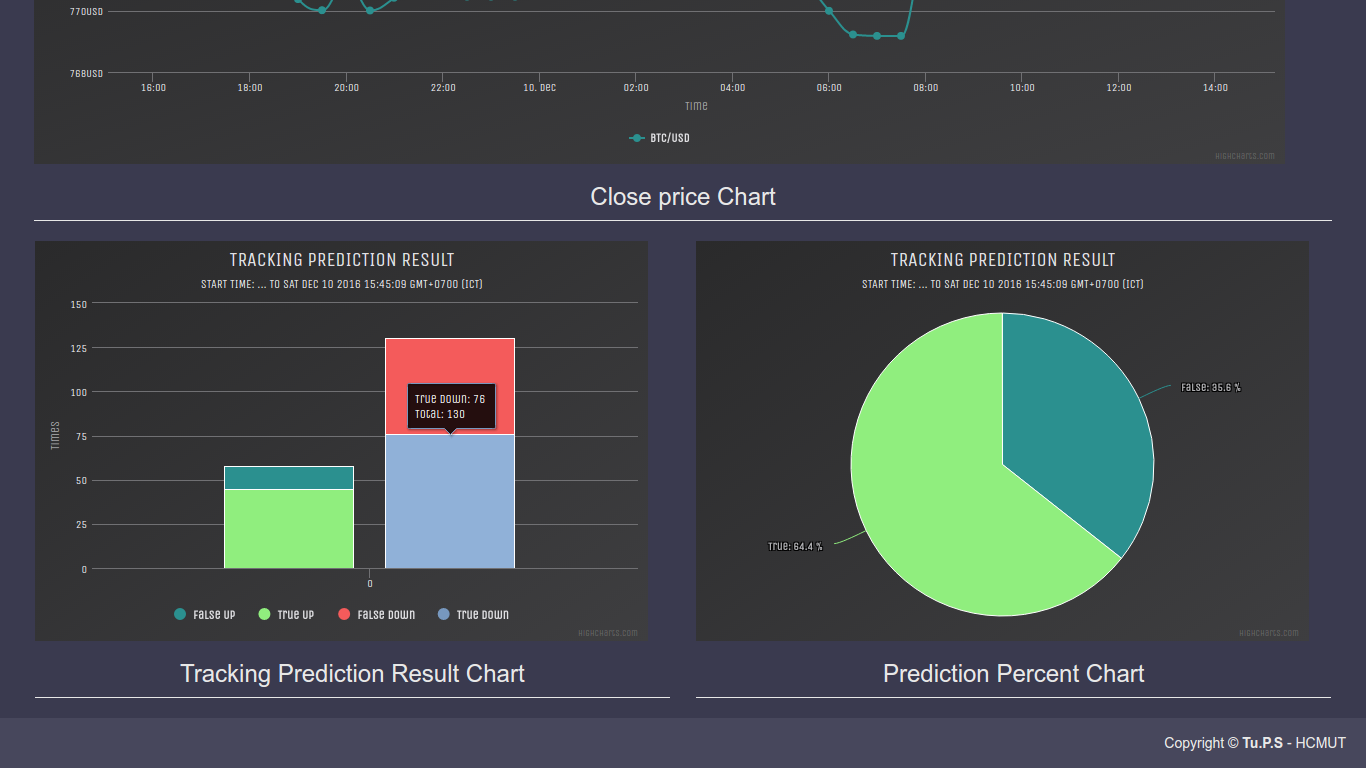
\includegraphics[height=3in, keepaspectratio=true]{3.png}
\caption{Giao diện 3 máy chủ UI frontend}
\end{figure}\\\\
Hệ thống máy chủ UI frontend được xây dựng theo xu hướng one-page, cũng chính 
vì vậy mà Angular 2 là lựa chọn phù hợp, với khả năng phát triển nhanh, hỗ trợ 
tốt từ các bên thứ 3.
\chapter{Kết luận và hướng phát triển}

\section{Kết luận}
Kết thúc đề tài, sản phẩm cuối cùng được hoàn thiện là một công cụ nền Web hỗ 
trợ, cung cấp các thông tin có giá trị tham khảo để đầu tư Bitcoin. Dựa trên 
các con số lý thuyết, khả năng dự đoán chính xác là rất khả quan và đặc biệt, 
giải thuật được tối ưu cho phù hợp với góc nhìn của một người đầu tư.\\\\
Với không nhiều sai lệch khi so sánh bên cạnh các con số lý thuyết, khi hệ thống được cho chạy 
thực tế trong vòng 4 ngày liên tiếp (Cụ thể từ 22:30:00 13/11/2016 đến 
20:30:00 17/11/2016) đã cho ra kết quả:\\
\begin{table}[h]
\centering
\begin{tabular}{ |c|c|c| }
\hline
Accuracy & Precision & Recall \\
\hline
64.4\% & 77.6\% & 45.5\% \\
\hline
\end{tabular}
\caption{Bảng đánh giá hệ thống thực tế }
\end{table}\\
Các tham số đánh giá chạy thực tế như vậy, có thể thấy với một lần đầu tư 
ta có tới hơn 70\% là có lợi nhuận. Tuy vậy, bất kỳ một hệ thống cũng vẫn 
sẽ có những điểm thiếu sót.\\\\
Vì giới hạn của thời gian thực hiện đề tài, phạm vi của đề tài cũng được thu 
hẹp để phù hợp nên vì thế đã bỏ qua một số yếu tố thị trường ảnh hưởng khá lớn 
đối với hướng giải quyết. Trong lúc này, bản thân có thể nhận ra hai vấn đề:
\begin{itemize}
\item Phí giao dịch: ở tất cả các sàn giao dịch, đều có một khoảng phí trung gian 
từ 0.1\% đến 0.3\% và phí này được trừ trực tiếp vào các giao dịch. Hướng tiếp 
cận của đề tài bỏ qua hoàn toàn yếu tố này và có thể hiểu là phí bằng 0\%
\item Biên độ lợi nhuận và thua lỗ: chúng ta cũng đã bỏ qua yếu tố này, mặc dù 
dựa theo đánh giá thì số lần đầu tư lợi nhuận sẽ nhiều hơn thua lỗ. Nhưng, chúng 
ta không thể kết luận việc đầu tư sẽ chắc chắn đem về lợi nhuận. Hãy nói đến một 
trường hợp xấu, biên độ lợi nhuận chỉ có \$1 cho mỗi lần nhưng biên độ thua lô 
lại là \$100, tại đây chúng ta có thể thấy là việc đầu tư không hề có lợi.
\end{itemize}
Việc nhìn nhận được các vấn đề trên không hẳn là điều tồi tệ, mà ngược lại giúp 
chúng ta có thể hiểu rõ bài toán và đưa ra những hướng phát triển tiếp theo.

\section{Hướng phát triển}
Với các vấn đề còn tồn tại được nêu ra bên trên (Mục 5.1), giai đoạn tiếp theo 
của đề tài là đi giải quyết vẫn đề tài như hiện giờ nhưng thêm vào đó là yếu 
tố phí giao dịch. Tuy là một yếu tố nhỏ nhưng nó dẫn đến việc thay đổi hoàn toàn 
bộ dữ liệu ban đầu, điều này đồng nghĩa toàn bộ hệ thống hiện giờ sẽ không 
tương thích. Vì thế, cần thực hiện lại quá trình xây dựng giải thuật từ đầu.\\\\
Mặc khác, việc chỉ học duy nhất từ tập dữ liệu về giá Bitcoin là không đủ để 
đưa ra một dự đoán chính xác cao. Ngày nay, mạng xã hội đang phát triển như vũ 
bão, đây là một kênh thông tin cực kỳ quý giá, chính vì vậy mà hệ thống ở giai 
đoạn phát triển tiếp theo sự tận dụng tài nguyên này.\\\\
Phát triển hệ thống xử lý ngôn ngữ tự nhiên, xây dựng hệ thống lắng nghe các 
thông tin tài chính, chính trị có ảnh hưởng tới giá trị Bitcoin, phân tích, 
đánh giá và cho cân bằng với hệ thống học từ dữ liệu giá Bitcoin để cho ra một 
dự đoán tổng quát và chính xác hơn.\\\\
Đồng thời, hệ thống có thể mở rộng ra cho nhiều cryptocurrency khác như Ethereum,
Zcash, Monero...
 
\pagebreak
\begin{thebibliography}{9}

\bibitem{Bitcoin}
Wikipedia. ``Bitcoin'' Internet: https://en.wikipedia.org/wiki/Bitcoin, Tháng 11/2016.
\bibitem{BitcoinPaper}
Satoshi Nakamoto. \emph{Bitcoin: A Peer-to-Peer Electronic Cash System}.
\bibitem{PredictingGoldPrices}
Megan Potoski. (2013) \emph{Predicting Gold Prices}. 
\bibitem{StockPriceTrendForecasting}
Yuqing Dai \& Yuning Zhang. (2013). \emph{Machine Learning in Stock Price Trend Forecasting}.
\bibitem{MachineLearningLec}
Andrew Ng. (2012).\emph{Lecture Notes – CS229 Machine Learning}.
\bibitem{MachineLearningSec}
Andrew Ng. (2012).\emph{Section Notes – CS229 Machine Learning}.
\bibitem{NeuralNetworksandDeepLearning}
Michael Nielsen. (2016, tháng 1). \emph{Neural Networks and Deep Learning - Free Online Book}.
\end{thebibliography}
\end{document}
